%%=============================================================================
%% Methodologie
%%=============================================================================

\chapter{\IfLanguageName{dutch}{Methodologie}{Methodology}}
\label{ch:methodologie}

%% TODO: Hoe ben je te werk gegaan? Verdeel je onderzoek in grote fasen, en
%% licht in elke fase toe welke stappen je gevolgd hebt. Verantwoord waarom je
%% op deze manier te werk gegaan bent. Je moet kunnen aantonen dat je de best
%% mogelijke manier toegepast hebt om een antwoord te vinden op de
%% onderzoeksvraag.

In dit hoofdstuk zal de gebruikte werkwijze van het onderzoek diepgaand uitgelegd worden met de nodige verantwoording.

Dit onderzoek stelt een werkwijze voor om handgeschreven karakters te classificeren per schriftsysteem aan de hand van een convolutioneel neuraal netwerk.
De gebruikte werkwijze bestaat uit verschillende fasen en komen in dit hoofdstuk aan bod.


\section{Data verzameling}

De eerste stap in de werkwijze van dit onderzoek was het nagaan welke datasets nodig waren om het model te trainen.
Het doel van het model is om handgeschreven karakters te classificeren per schriftsysteem, hiervoor waren verschillende datasets van meerdere schriftsystemen nodig, deze bestaande uit afbeelding van handgeschreven karakters.

Een grote factor die invloed had op de keuze van de schriftsystemen lag bij de beschikbaarheid van datasets van het schriftsysteem.
Wanneer een potentieel schriftsysteem werd gekozen moest het toeval er bij liggen dat er een dataset bestond waarbij de data bruikbaar was en uit voldoende data bestond.
Als de dataset niet voldeed aan de eisen werd de dataset achterwege gelaten.
Vervolgens werd er of naar een andere dataset gezocht of werd het schriftsysteem niet gebruikt.



Geweten is dat er 3 grote groepen zijn bij de schriftsystemen, het lag voor de hand om één schriftsysteem te gebruiken per groep.

Het eerste schriftsysteem dat voldeed aan de eisen was het Latijns schrift, dit onder de CoMNIST dataset.
De dataset is een online dataset aangezien de data wordt verzameld door middel van een webapplicatie waar iedereen aan kan participeren.
Deze dataset bestaat uit twee mappen, één daarvan is het Latijns schrift, de andere is het Cyrillisch schrift dat in dit onderzoek niet gebruikt zal worden.
Het Latijns schrift wordt vooral gebruikt in de westerse wereld, dit is de reden waarom het een eerste en simpele keuze was.
Dit schrift valt onder de alfabetische groep en vult al één van de drie plaatsen op.

De tweede plaats werd opgevuld door het Kanji, één van de schriften gebruikt in het Japans.
Dit schrift valt onder de logografische groep en is daardoor een goede tweede keuze.
De naam van de dataset is de Kuzushiji-MNIST dataset, een offline dataset.
Deze bestaat uit drie verschillende mappen, enkel de Kuzishiji-Kanji werd gebruikt aangezien dit het grootste aantal aan verschillende karakters bevatte.
Dit zou een voordeel bieden voor het trainen van het model.

Voor de laatste plaats werd er een syllabisch schrift gekozen.
Het gekozen schrift was het Arabisch, een gekend lettergrepenschrift dat in vooral in de Arabische wereld wordt gebruikt.
Een dataset in het bezit van \autocite{Ahmed2017}, bestaande uit een groot aantal Arabische karakters.

\section{Data voorbereiding}

Twee van de drie gekozen datasets zijn bedoeld voor het herkennen van de karakters onder het schriftsysteem van de dataset.
Deze datasets bestonden daardoor uit een structuur van mappen waarbij elke map een specifiek karakter voorstelde uit het schriftsysteem, in elke map zaten vervolgens alle afbeeldingen toebehorend aan dat karakter.

Aangezien in dit onderzoek enkel gezocht werd naar het bijhorende schriftsysteem was het voordelig dat alle afbeeldingen in één grote map zaten.
Er werd hier gesproken over meer dan 10.000 afbeeldingen, deze allen verplaatsen met windows file explorer was geen goede keuze.
Voor deze data verplaatsing werd er eens bash script geschreven dat alles verplaatste. (Tabel \ref{table:BashScript})

\begin{table}[!htbp]
    \begin{tabular}{|l|}
        \hline
        \begin{lstlisting}
find . -mindepth 2 -type f -print -exec mv {} . \;
        \end{lstlisting}
        \\ \hline
    \end{tabular}
    \caption{Bash script voor alle data in één map te verplaatsen. }\label{table:BashScript}
\end{table}

Wanneer al de data voldoende was gestructureerd was het klaar voor de manipulaties die nodig waren voor gebruik.

De datamanipulatie werd gedaan in python, hier waren verschillende libraries voor gebruikt, genaamd numpy, matplotlib, os, tqdm en cv2.
Wanneer een model getraind wordt aan de hand van een groot aantal verschillende afbeelding moeten de afbeelding allen dezelfde afmetingen bevatten, de keuze voor de hoogte en breedte had invloed op het detailgehalte van de afbeelding, wanneer een lage waarde werd gekozen was er weinig detail te zien, bij een grote waarde was er meer detail te zien.
Voor de afmeting van de afbeeldingen die gebruikt werden bij het model werd een waarde van 60 genomen. (Figuur \ref{tab:afmetingen})


\begin{figure}
    
    
    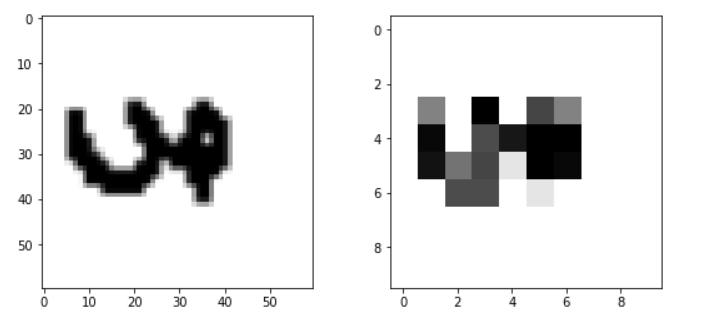
\includegraphics[width=\linewidth]{img/Afmetingen.png}

    \caption{verschil tussen een waarde van 60 (60x60) en een waarde van 10 (10x10) voorgesteld door een Arabisch karakter uit de gebruikte data.}
    \label{tab:afmetingen}
    
\end{figure}

Bij een classificatieprobleem, waar dit onderzoek mee kampt, worden de klassen voorgesteld door numerieke waarden (0, 1, 2, ...). Deze numerieke waarden worden labels genoemd.
Vervolgens worden de afbeeldingen gelinkt aan de bijhorende numerieke waarde.
Bij dit onderzoek zijn de numerieke waarden de schriftsystemen.
Voor het vergemakkelijken voor het model om de data te begrijpen werd er voor gezorgd dat de afbeeldingen allen zwart op wit stonden, de Kanji dataset is bijvoorbeeld wit op zwart dit werd gecorrigeerd.
Als voorlaatste stap werden de afbeeldingen omgezet naar twee-dimensionale matrices waarbij elke waarde in de matrix een waarde voorstelde van de pixel op die positie in de afbeelding.
Uiteindelijk werd de matrix in een lijst geplaatst met de bijhorende label (de numerieke waarde die het schriftsysteem voorstelt). (Tabel \ref{table:DataManipulation})


\begin{table}[!htbp]
    \begin{tabular}{|l|}
        \hline
        \begin{lstlisting}
training_data = []
def create_train_data():
   for category in CATEGORIES: 
      path = os.path.join(DATADIR,category) 
        class_num = CATEGORIES.index(category)
        for img in tqdm(os.listdir(path)): 
          try:
             if(category == "Kanji"):
                 img_array = cv2.imread(
                    os.path.join(path,img),cv2.IMREAD_GRAYSCALE) 
             else:
                 img_array = cv2.bitwise_not(cv2.imread(
                    os.path.join(path,img),cv2.IMREAD_GRAYSCALE))
             new_arr = cv2.resize(img_array,(IMG_SIZE,IMG_SIZE))
             training_data.append([new_arr, class_num])
           except Exception as e:
             pass
        \end{lstlisting}
        \\ \hline
    \end{tabular}
    \caption{Python code voor de manipulatie van de gebruikte datasets (CATEGORIES zijn de gebruikte schriftsystemen) }\label{table:DataManipulation}
\end{table}

De data werd vervolgens willekeurig door elkaar geschud en opgesplitst in twee verschillende lijsten, een lijst van de matrices die de afbeelding voorstelt en een lijst van de bijhorende labels. De positie van een afbeelding in de lijst van matrices ligt op dezelfde positie als de bijhorende label in de andere lijst.
Om de verwerkte data op te slaan werd pickle gebruikt (Tabel \ref{table:DataSave})


\begin{table}[!htbp]
    \begin{tabular}{|l|}
        \hline
        \begin{lstlisting}
import pickle
       
pickle_out = open("X.pickle","wb")
pickle.dump(X, pickle_out)
pickle_out.close()
        \end{lstlisting}
        \\ \hline
    \end{tabular}
    \caption{Het opslaan van de verwerkte data in python door middel van pickle }\label{table:DataSave}
\end{table}

\section{Het Convolutioneel Neuraal Netwerk}

Het ontwerpen van een neuraal netwerk is een proces van trial-and-error.
Een eerste model wordt ontworpen, getraind en als laatste getest, wanneer de accuraatheid van het model niet hoog ligt wordt er gekeken naar het ontwerp van het model.
Er wordt gekeken of er enige aanpassingen nodig zijn voor het verbeteren van de resultaten, wanneer de accuraatheid hoger ligt dan voorheen wordt op dit model verder gewerkt.
Uiteindelijk wordt er een model ontwikkeld dat het best past bij het classificatieprobleem.
In dit hoofdstuk wordt het model besproken dat het best past bij het onderzoek, alsook de verantwoording voor de structuur van het model.

Het model werd ontworpen in python. Voor de implementatie van alle lagen, het laten trainen en testen met de voorbereide data werd tensorflow gebruikt, een open source platform die zich specialiseert in machine learning.
In python werd de library ingeladen zodat de nodige lagen voor een convolutioneel neuraal netwerk gebruikt konden worden.

Aangezien het neuraal netwerk waarden inleest tussen 0 en 1 werden de waarden in de lijst van de lijst van matrices genormaliseerd.
Vervolgens werd de data opgesplitst in traindata waarop het model werd getraind en testdata waarop de accuraatheid van het model werd getest.  \ref{table:DataNormalisition}



\begin{table}[!htbp]
    \begin{tabular}{|l|}
        \hline
        \begin{lstlisting}
X = pickle.load(open("X.pickle","rb"))
y = pickle.load(open("y.pickle","rb"))
       
X = X/255.0

X_train, X_test, y_train, y_test =
       train_test_split(X,y,test_size=0.2)
        \end{lstlisting}
        \\ \hline
    \end{tabular}
    \caption{Het inladen en normaliseren van de data en het opsplitsen van de data} }\label{table:DataNormalisition}
\end{table}


Een model wordt aangemaakt en de nodige lagen worden er aan toegevoegd, als eerste laag werd een convolutionele laag geplaatst in het model.
Voor deze laag zijn een aantal parameters nodig, als eerste wordt het aantal filters gevraagd. 
Het aantal filters bepaald ook het aantal neuronen in de laag, want elke filter is verbonden met een neuron.
De keuze voor het aantal filters ligt bij hoeveel karakteristieken er herkend willen worden, aangezien het de eerste laag is werd een aantal van 32 filters gekozen.

Als tweede parameter werd de afmeting gevraagd voor de filter.
De keuze voor de afmeting wordt bepaald door welke soort karakteristieken de filters moeten kunnen verwerken. Wanneer er veel detail in de afbeelding aanwezig is zullen er kleinere afmetingen worden meegegeven, als er grotere karakteristieken moet herkend worden waar weinig detail aan te pas komt zullen er grotere afmetingen worden meegegeven.
Aangezien de eerste laag vooral simpele karakteristieken zoals vormen, krommingen, et cetera moeten herkend worden werd er een afmeting van 5x5 meegegeven.
Als er geweten is dat de kleinst mogelijke filter een afmeting van 3x3 bevat zorgt de gekozen afmeting van 5x5 voor het leren van gedetailleerde karakteristieken maar meer rekening houdend met omliggende factoren.

Een derde parameter dat wordt gevraagd is de activatiefunctie, de activatiefunctie bepaalt de uitvoer van de laag.
Voor deze laag werd 'Relu', ook wel 'Rectified linear unit' genoemd, gekozen.

        $f(x) = x^+ = max(0,x)$

Deze functie veranderd alle negatieve waarden naar 0 en de positieve waarden blijven hun waarde behouden.
Wanneer deze functie wordt uitgevoerd op een afbeelding blijven enkel de grijze en witte waarden over, de zwarte waarden worden vervangen.
Door deze activatiefunctie wordt het trainingsproces versneld.
(Figuur \ref{tab:Relu})

\begin{figure}
    
    
    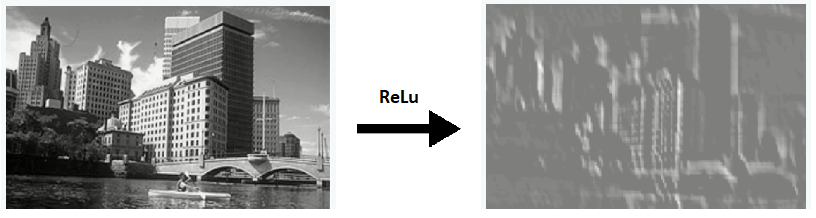
\includegraphics[width=\linewidth]{img/ReLu.png}
    
    \caption{ReLu functie uitgevoerd op een afbeelding.}
    \label{tab:Relu}
    
\end{figure}

Bij de eerste laag in een convolutioneel neuraal netwerk wordt de afmeting gevraagd van de matrices die in de inputlaag zullen worden meegegeven. 

\begin{table}[!htbp]
    \begin{tabular}{|l|}
        \hline
        \begin{lstlisting}
model.add(
    Conv2D(32, (5, 5), activation='relu',input_shape=X.shape[1:]))
model.add(
    MaxPooling2D((2, 2)))

        \end{lstlisting}
        \\ \hline
    \end{tabular}
    \caption{Een eerste convolutioneele laag en een pooling laag} }\label{table:FirstLayers}\end{table}

Nadat een convolutionele laag is toegevoegd aan het model wordt er een pooling laag achter geplaatst.
Bij de pooling laag zijn de verwachte parameters de afmeting van de filter.
Een afmeting van 2x2 werd meegegeven, De gekozen pooling laag is de max pooling laag.

 














